\documentclass[11pt,a4paper]{article}
\usepackage[margin=21mm,headheight=16pt]{geometry}
\usepackage{fontspec}\setmainfont{Noto Serif}\setsansfont{Noto Sans}\setmonofont{Noto Sans Mono}
\usepackage{polyglossia}\setdefaultlanguage{turkish}
\usepackage{amsmath,amssymb,mathtools,graphicx,xcolor,booktabs,tabularx,array,enumitem}
\usepackage[most]{tcolorbox}\usepackage{fancyhdr,titlesec,needspace}
\usepackage[unicode,hidelinks,breaklinks]{hyperref}\usepackage{bookmark}
\definecolor{ink}{HTML}{18233A}\definecolor{accent}{HTML}{545AC4}\definecolor{green}{HTML}{087E66}\definecolor{paper}{HTML}{F3F5FA}
\color{ink}\setlength{\parindent}{0pt}\setlength{\parskip}{7pt}\linespread{1.10}
\setlength{\emergencystretch}{3em}\allowdisplaybreaks
\setlist{topsep=4pt,itemsep=4pt,leftmargin=*}
\pagestyle{fancy}\fancyhf{}\fancyhead[L]{\sffamily\small MÜHENDİSLİK MATEMATİĞİ}\fancyhead[R]{\sffamily\small Ders çalışma notları}\fancyfoot[L]{\sffamily\scriptsize Fotoğraflar + müfredat | 8 Kasım 2026}\fancyfoot[R]{\sffamily\thepage}
\titleformat{\section}{\Large\sffamily\bfseries\color{accent}}{\thesection}{.6em}{}
\titleformat{\subsection}{\large\sffamily\bfseries}{\thesubsection}{.6em}{}
\tcbset{enhanced,breakable,boxrule=.4pt,arc=2mm,left=3mm,right=3mm,top=2mm,bottom=2mm,before skip=8pt,after skip=8pt,fonttitle=\sffamily\bfseries,colback=paper,colframe=accent,coltitle=white}
\newcommand{\notebox}[2]{\begin{tcolorbox}[title={#1},colframe=accent!70!black]#2\end{tcolorbox}}
\hypersetup{pdfauthor={Mühendislik Matematiği Çalışma Atölyesi},pdfsubject={Ders fotoğrafları ve altı başlıklı müfredata göre özgün Türkçe çalışma notları}}
\begin{document}

\hypersetup{pdftitle={Kısmi türev, teğet düzlem ve lineer yaklaşım}}
{\sffamily\small\color{accent} ÇALIŞMA ATÖLYESİ / KONU 05\par}
\vspace{8mm}
{\Huge\sffamily\bfseries\raggedright\hyphenpenalty=10000 Kısmi türev, teğet düzlem ve lineer yaklaşım\par}
\vspace{3mm}
{\large Kısmi ve karma türevler, türevlenebilirlik, diferansiyel, lineerleştirme ve hata sınırı.\par}
\vspace{4mm}\hrule\vspace{4mm}\subsection*{Bu bölümün hedefleri}\begin{itemize}
\item Kısmi türev alırken hangi değişkenin sabit tutulduğunu açıklamak.
\item Kısmi türevlerin varlığı ile türevlenebilirliği ayırt etmek.
\item Teğet düzlem, diferansiyel ve lineer yaklaşımı hata sınırıyla kullanmak.\end{itemize}
{\small\tableofcontents}\clearpage
\section{Kısmi türev: tek yöndeki değişim}
İki değişkenli bir fonksiyonda x değişirken y sabit tutulursa tek değişkenli bir kesit elde edilir. Bu kesitin türevi \(f_x\) olur. Benzer biçimde y değişirken x sabit tutularak \(f_y\) bulunur. Sabit tutmak, diğer değişkeni sıfır yapmak demek değildir; türev sırasında katsayı gibi davranmasını sağlamaktır.


{\small\[
f_x(a,b)=\lim_{h\to0}\frac{f(a+h,b)-f(a,b)}h,\qquad f_y(a,b)=\lim_{h\to0}\frac{f(a,b+h)-f(a,b)}h.
\]}
\Needspace{10\baselineskip}\begin{tcolorbox}[title={Örnek 5.1 | Dersteki temel kısmi türev},colframe=accent]\(f(x,y)=x^2y^3+3x\) için birinci kısmi türevleri bulunuz.
\par\vspace{1mm}{\scriptsize\sffamily Ders fotoğrafından | \nolinkurl{IMG-20261022-WA0055.jpg}}\end{tcolorbox}
\begin{tcolorbox}[title={Adım adım çözüm},colback=green!3!white,colframe=green]\begin{enumerate}
\item x yönünde y sabittir: \(f_x=2xy^3+3\). y yönünde x sabittir: \(f_y=3x^2y^2\).
\item Örneğin \((1,2)\) noktasında \(f_x=19\), \(f_y=12\). Bunlar yüzeyin koordinat kesitlerindeki eğimleridir.
\end{enumerate}\end{tcolorbox}
\Needspace{10\baselineskip}\begin{tcolorbox}[title={Örnek 5.2 | Limit tanımıyla kısmi türev},colframe=accent]\(f(x,y)=x^2y\) için \(f_x(a,b)\) değerini tanımdan bulunuz.
\par\vspace{1mm}{\scriptsize\sffamily Pekiştirme}\end{tcolorbox}
\begin{tcolorbox}[title={Adım adım çözüm},colback=green!3!white,colframe=green]\begin{enumerate}
\item \([f(a+h,b)-f(a,b)]/h=[(a+h)^2b-a^2b]/h=2ab+bh\).
\item h sıfıra giderken \(f_x(a,b)=2ab\) elde edilir. Bu, diğer değişkeni neden sabit tuttuğumuzu doğrudan gösterir.
\end{enumerate}\end{tcolorbox}
\section{Yüksek mertebeli ve karma türevler}
Birinci kısmi türevler de fonksiyon olduğundan yeniden türevlenebilir. Bu notlarda \(f_{xy}=(f_x)_y\): önce x, sonra y türevi demektir. İşlem sırasını açık yazmak farklı kaynaklardaki gösterim karışıklığını önler. Karma türevler bir komşulukta sürekli ise Clairaut-Schwarz teoremi \(f_{xy}=f_{yx}\) verir.


{\small\[
f_{xx}=\frac{\partial^2 f}{\partial x^2},\quad f_{xy}=\frac{\partial}{\partial y}\left(\frac{\partial f}{\partial x}\right),\quad f_{yx}=\frac{\partial}{\partial x}\left(\frac{\partial f}{\partial y}\right),\quad f_{yy}=\frac{\partial^2f}{\partial y^2}.
\]}
\Needspace{10\baselineskip}\begin{tcolorbox}[title={Örnek 5.3 | Dersteki rasyonel fonksiyonun ikinci türevleri},colframe=accent]\(f(x,y)=xy/(x^2+y^2)\), \((x,y)\ne(0,0)\) için ikinci kısmi türevleri bulunuz.
\par\vspace{1mm}{\scriptsize\sffamily Ders fotoğrafından | \nolinkurl{IMG-20261022-WA0055.jpg}}\end{tcolorbox}
\begin{tcolorbox}[title={Adım adım çözüm},colback=green!3!white,colframe=green]\begin{enumerate}
\item \(S=x^2+y^2\) kısaltmasıyla bölüm kuralından \(f_x=y(y^2-x^2)/S^2\), \(f_y=x(x^2-y^2)/S^2\).
\item \(f_{xx}\) için \(-2xy/S^2-4xy(y^2-x^2)/S^3\) ortak paydada toplanır: \(f_{xx}=2xy(x^2-3y^2)/S^3\).
\item Simetriyle \(f_{yy}=2xy(y^2-3x^2)/S^3\). Karma türev \(f_{xy}=(-x^4+6x^2y^2-y^4)/S^3\).
\item Orijin dışında türevler süreklidir; \(f_{yx}=f_{xy}\). Orijinde başlangıç fonksiyonu tanımlı olmadığı için bu formüller orijine uygulanmaz.
\end{enumerate}\end{tcolorbox}
\notebox{Teoremin koşulları}{Karma türevlerin eşitliğini koşulsuz kabul etme. Sürekli ikinci kısmi türevler yeterli bir koşuldur; parçalı tanımlı fonksiyonlarda ayrı kontrol gerekebilir.}
\section{Türevlenebilirlik neden daha güçlüdür?}
Kısmi türevler iki özel yönü ölçer. Türevlenebilirlik ise noktanın çevresindeki tüm küçük değişimlerin aynı lineer fonksiyonla açıklanabilmesini ister. Hata, yer değiştirmenin uzunluğuna göre ihmal edilebilir olmalıdır. Bu koşul teğet düzlemin yüzeyi yerel olarak temsil etmesini sağlar.


{\small\[
f(a+h,b+k)=f(a,b)+f_x(a,b)h+f_y(a,b)k+R(h,k),\quad\frac{R(h,k)}{\sqrt{h^2+k^2}}\to0.
\]}
\(f_x,f_y\) bir komşulukta var ve noktada sürekli ise f o noktada türevlenebilirdir. Türevlenebilirlik sürekliliği ve kısmi türevlerin varlığını gerektirir. Ters yöndeki çıkarımlar tek başlarına doğru değildir.

\Needspace{10\baselineskip}\begin{tcolorbox}[title={Örnek 5.4 | Kısmi türevler var, süreklilik yok},colframe=accent]\(f(x,y)=xy/(x^2+y^2)\) orijin dışında, \(f(0,0)=0\) olsun. Orijinde kısmi türevleri ve türevlenebilirliği inceleyiniz.
\par\vspace{1mm}{\scriptsize\sffamily Pekiştirme}\end{tcolorbox}
\begin{tcolorbox}[title={Adım adım çözüm},colback=green!3!white,colframe=green]\begin{enumerate}
\item Eksenler boyunca fonksiyon sıfırdır. Bu yüzden \(f_x(0,0)=f_y(0,0)=0\).
\item \(y=x\) boyunca değer \(1/2\), dolayısıyla fonksiyon orijinde sürekli değildir. Sürekli olmayan fonksiyon türevlenebilir olamaz.
\end{enumerate}\end{tcolorbox}
\section{Teğet düzlem ve normal doğru}
\(z=f(x,y)\) grafiğinde \(P=(a,b,f(a,b))\) noktasındaki iki teğet yön \((1,0,f_x)\) ve \((0,1,f_y)\) olur. Çarpımları \((-f_x,-f_y,1)\) normalini verir. Yeterli türevlenebilirlik koşulları altında bu normal teğet düzlemi belirler.


{\small\[
z-f(a,b)=f_x(a,b)(x-a)+f_y(a,b)(y-b).
\]}

{\small\[
\text{Normal doğru: }\ (x,y,z)=(a,b,f(a,b))+t(-f_x(a,b),-f_y(a,b),1).
\]}
\Needspace{10\baselineskip}\begin{tcolorbox}[title={Örnek 5.5 | Teğet düzlem ve lineer model},colframe=accent]\(f(x,y)=x^2+y^2\) için \((1,2,5)\) noktasındaki teğet düzlemi ve normal doğruyu bulunuz.
\par\vspace{1mm}{\scriptsize\sffamily Pekiştirme}\end{tcolorbox}
\begin{tcolorbox}[title={Adım adım çözüm},colback=green!3!white,colframe=green]\begin{enumerate}
\item \(f_x=2x,f_y=2y\). Noktadaki eğimler 2 ve 4. Düzlem \(z-5=2(x-1)+4(y-2)\), yani \(z=2x+4y-5\).
\item Normal doğru \((x,y,z)=(1,2,5)+t(-2,-4,1)\). Normalin işaretini ters almak aynı doğruyu verir.
\end{enumerate}\end{tcolorbox}
\begin{center}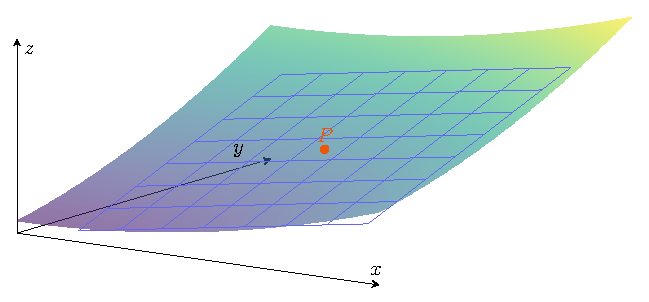
\includegraphics[width=.94\linewidth,height=65mm,keepaspectratio]{../assets/figures/tangent.pdf}\par{\small\sffamily Yüzey ile teğet düzlem, temas noktası yakınında aynı birinci mertebe değişimi verir.}\end{center}
\section{Lineerleştirme ve yaklaşık değer}
Lineerleştirme \(L(x,y)\), teğet düzlemin z değeri olarak okunan afin fonksiyondur. Hesabı kolay bir merkez seçilir; merkezdeki fonksiyon değeri ve türevler bulunur; hedef noktanın küçük farkları formüle konur. Yaklaşımın güvenilirliği, merkeze uzaklık ve ikinci türevlerin büyüklüğüne bağlıdır.


{\small\[
L(x,y)=f(a,b)+f_x(a,b)(x-a)+f_y(a,b)(y-b),\qquad f(x,y)\approx L(x,y).
\]}
\Needspace{10\baselineskip}\begin{tcolorbox}[title={Örnek 5.6 | Dersteki üstel fonksiyonun iki lineerleştirmesi},colframe=accent]\(f(x,y)=e^{2y-x}\) için \(P=(0,0)\) ve \(Q=(1,2)\) merkezlerindeki lineerleştirmeleri bulunuz.
\par\vspace{1mm}{\scriptsize\sffamily Ders fotoğrafından | \nolinkurl{IMG-20261105-WA0038.jpg}}\end{tcolorbox}
\begin{tcolorbox}[title={Adım adım çözüm},colback=green!3!white,colframe=green]\begin{enumerate}
\item \(f_x=-e^{2y-x}\), \(f_y=2e^{2y-x}\). P merkezinde \(L_P=1-x+2y\).
\item Q merkezinde \(f=e^3,f_x=-e^3,f_y=2e^3\). Bu yüzden \(L_Q=e^3-e^3(x-1)+2e^3(y-2)=e^3(2y-x-2)\).
\item Her model kendi merkezinin yakınında kullanılır. Örneğin \(f(0.01,0.02)=e^{0.03}\approx1.03\); bu hedef P merkezine yakındır.
\end{enumerate}\end{tcolorbox}
\Needspace{10\baselineskip}\begin{tcolorbox}[title={Örnek 5.7 | Karekökün yaklaşık değeri},colframe=accent]\(\sqrt{(3.01)^2+(3.98)^2}\) ifadesini diferansiyel veya lineer modelle yaklaşık hesaplayınız.
\par\vspace{1mm}{\scriptsize\sffamily Pekiştirme}\end{tcolorbox}
\begin{tcolorbox}[title={Adım adım çözüm},colback=green!3!white,colframe=green]\begin{enumerate}
\item \(f(x,y)=\sqrt{x^2+y^2}\), merkez \((3,4)\), \(f=5\). \(f_x=3/5,f_y=4/5\).
\item \(h=0.01,k=-0.02\). Yaklaşık değer \(5+(3/5)(0.01)+(4/5)(-0.02)=4.99\).
\end{enumerate}\end{tcolorbox}
\section{Lineer yaklaşımın hata sınırı}
İkinci türevler merkezi hedefe bağlayan parçayı içeren bir bölgede sürekli ve \(|f_{xx}|\le M\), \(|f_{xy}|\le M\), \(|f_{yy}|\le M\) olsun. Tek değişkenli Taylor teoremi \(g(t)=f(a+th,b+tk)\) fonksiyonuna uygulanırsa aşağıdaki güvenli üst sınır elde edilir. M yalnızca merkezdeki değer değildir; bütün ilgili bölgede geçerli olmalıdır.


{\small\[
|f(a+h,b+k)-L(a+h,b+k)|\le\frac M2(|h|+|k|)^2.
\]}
\Needspace{10\baselineskip}\begin{tcolorbox}[title={Örnek 5.8 | Defterdeki hata sınırı},colframe=accent]\(f=x^2+3xy+2y^2+4\), merkez \((2,1)\), \(|x-2|,|y-1|\le0.01\). Lineerleştirmeyi ve hata sınırını bulunuz.
\par\vspace{1mm}{\scriptsize\sffamily Ders fotoğrafından | \nolinkurl{IMG-20261022-WA0060.jpg}}\end{tcolorbox}
\begin{tcolorbox}[title={Adım adım çözüm},colback=green!3!white,colframe=green]\begin{enumerate}
\item \(f(2,1)=16\), \(f_x(2,1)=7\), \(f_y(2,1)=10\). \(L=16+7(x-2)+10(y-1)=7x+10y-8\).
\item \(f_{xx}=2,f_{xy}=3,f_{yy}=4\). M=4 seçilir; hata en fazla \(\tfrac42(0.01+0.01)^2=0.0008\).
\item Kontrol: gerçek kalan \(h^2+3hk+2k^2\) olur. Mutlak değer için daha sıkı \(0.0006\) sınırı da mümkündür; dersteki \(0.0008\) güvenli ve doğrudur.
\end{enumerate}\end{tcolorbox}
\Needspace{10\baselineskip}\begin{tcolorbox}[title={Örnek 5.9 | İkinci hata sınırı sorusu},colframe=accent]\(f=x^2-3xy+y^2\), merkez \((1,2)\), \(|x-1|,|y-2|\le0.1\). L ve güvenli hata sınırını bulunuz.
\par\vspace{1mm}{\scriptsize\sffamily Ders fotoğrafından | \nolinkurl{IMG-20261105-WA0038.jpg}}\end{tcolorbox}
\begin{tcolorbox}[title={Adım adım çözüm},colback=green!3!white,colframe=green]\begin{enumerate}
\item \(f(1,2)=-1,f_x=-4,f_y=1\) olduğundan \(L=-1-4(x-1)+(y-2)=-4x+y+1\).
\item İkinci türevlerin mutlak değerleri 2,3,2; M=3. Hata \(\le(3/2)(0.1+0.1)^2=0.06\).
\end{enumerate}\end{tcolorbox}
\Needspace{10\baselineskip}\begin{tcolorbox}[title={Örnek 5.10 | Küçük bölgede kosinüs hatası},colframe=accent]\(f(x,y)=1+x+\cos y\), merkez \((0,0)\), \(|x|,|y|\le0.2\). L ve hata sınırını bulunuz.
\par\vspace{1mm}{\scriptsize\sffamily Ders fotoğrafından | \nolinkurl{IMG-20261105-WA0040.jpg}}\end{tcolorbox}
\begin{tcolorbox}[title={Adım adım çözüm},colback=green!3!white,colframe=green]\begin{enumerate}
\item \(f(0,0)=2,f_x=1,f_y(0,0)=0\). Böylece \(L=2+x\).
\item \(f_{xx}=f_{xy}=0,|f_{yy}|=|\cos y|\le1\). Genel sınır 0.08 verir; yalnız y yönündeki gerçek ikinci terim kullanılırsa \(|f-L|=|\cos y-1|\le y^2/2\le0.02\).
\end{enumerate}\end{tcolorbox}
\section{Tam diferansiyel ve gerçek artış}
Gerçek artış \(\Delta f=f(a+\Delta x,b+\Delta y)-f(a,b)\) tam farktır. Diferansiyel \(df=f_x\,dx+f_y\,dy\) bu farkın lineer kısmıdır. Yaklaşık hesapta \(dx=\Delta x,dy=\Delta y\) alınır; buna rağmen \(df\) ve \(\Delta f\) genel olarak eşit değildir. Üç değişkende \(dw=f_xdx+f_ydy+f_zdz\).

\Needspace{10\baselineskip}\begin{tcolorbox}[title={Örnek 5.11 | Tahtadaki silindir hacmi değişimi},colframe=accent]Yarıçapı 3 cm, yüksekliği 10 cm olan silindirde yarıçap 0.01 cm artsın, yükseklik 0.1 cm azalsın. Hacim değişimini yaklaşık bulunuz.
\par\vspace{1mm}{\scriptsize\sffamily Ders fotoğrafından | \nolinkurl{IMG-20261108-WA0066.jpg}}\end{tcolorbox}
\begin{tcolorbox}[title={Adım adım çözüm},colback=green!3!white,colframe=green]\begin{enumerate}
\item \(V=\pi r^2h\); \(dV=2\pi rh\,dr+\pi r^2\,dh\). \(dr=0.01,dh=-0.1\).
\item \(dV=60\pi(0.01)+9\pi(-0.1)=-0.3\pi\) santimetre küp. Başlangıç hacmi \(90\pi\), yeni hacim yaklaşık \(89.7\pi\).
\item Tam değer \(\pi(3.01)^2(9.9)=89.69499\pi\). Yaklaşık ve tam değer arasındaki fark \(0.00501\pi\); yüksek mertebeli terimlerden gelir.
\end{enumerate}\end{tcolorbox}
\Needspace{10\baselineskip}\begin{tcolorbox}[title={Örnek 5.12 | Silindir için ikinci ders sorusu},colframe=accent]Yarıçap 10 cm den 9.9 cm ye, yükseklik 30 cm den 30.3 cm ye değişiyor. Yaklaşık hacim değişimi nedir?
\par\vspace{1mm}{\scriptsize\sffamily Ders fotoğrafından | \nolinkurl{IMG-20261108-WA0083.jpg}}\end{tcolorbox}
\begin{tcolorbox}[title={Adım adım çözüm},colback=green!3!white,colframe=green]\begin{enumerate}
\item \(dr=-0.1,dh=0.3\). \(dV=2\pi(10)(30)(-0.1)+\pi(100)(0.3)=-30\pi\) santimetre küp.
\item Başlangıç hacmi \(3000\pi\), yeni hacim yaklaşık \(2970\pi\). İşaret hacmin azaldığını gösterir.
\end{enumerate}\end{tcolorbox}
\section{İkinci tam diferansiyel ve Hessian}
Bağımsız \(dx,dy\) artışları sabit kabul edilerek bir kez daha diferansiyel alınır. Karma terim iki kez geldiği için katsayı 2 olur. \(d^2f\), karesi alınmış \(df\) değildir. İkinci mertebe Taylor yaklaşımında bu terimin yarısı kullanılır.


{\small\[
d^2f=f_{xx}dx^2+2f_{xy}dx\,dy+f_{yy}dy^2,\qquad f(a+h,b+k)\approx f+df+\frac12d^2f.
\]}

{\small\[
d^2w=w_{xx}dx^2+w_{yy}dy^2+w_{zz}dz^2+2w_{xy}dx\,dy+2w_{xz}dx\,dz+2w_{yz}dy\,dz.
\]}
\Needspace{10\baselineskip}\begin{tcolorbox}[title={Örnek 5.13 | Tahtadaki polinom diferansiyeli},colframe=accent]\(f=x^3+5xy^2+3xy+4x-3y+5\) için df ve ikinci diferansiyeli yazınız.
\par\vspace{1mm}{\scriptsize\sffamily Ders fotoğrafından | \nolinkurl{IMG-20261108-WA0082.jpg}}\end{tcolorbox}
\begin{tcolorbox}[title={Adım adım çözüm},colback=green!3!white,colframe=green]\begin{enumerate}
\item \(f_x=3x^2+5y^2+3y+4\), \(f_y=10xy+3x-3\). df bu katsayılarla dx ve dy nin toplamıdır.
\item \(f_{xx}=6x,f_{xy}=10y+3,f_{yy}=10x\). Dolayısıyla \(d^2f=6x\,dx^2+2(10y+3)dx\,dy+10x\,dy^2\).
\end{enumerate}\end{tcolorbox}
\Needspace{10\baselineskip}\begin{tcolorbox}[title={Örnek 5.14 | Üç değişkenli polinomun diferansiyelleri},colframe=accent]\(w=3x^2yz^2-3xy+2yz^2+xyz\) için birinci ve ikinci diferansiyeli bulunuz.
\par\vspace{1mm}{\scriptsize\sffamily Ders fotoğrafından | \nolinkurl{IMG-20261108-WA0082.jpg}}\end{tcolorbox}
\begin{tcolorbox}[title={Adım adım çözüm},colback=green!3!white,colframe=green]\begin{enumerate}
\item \(w_x=6xyz^2-3y+yz\), \(w_y=3x^2z^2-3x+2z^2+xz\), \(w_z=6x^2yz+4yz+xy\). \(dw=w_xdx+w_ydy+w_zdz\).
\item \(w_{xx}=6yz^2,w_{yy}=0,w_{zz}=6x^2y+4y\). Karma türevler \(w_{xy}=6xz^2-3+z\), \(w_{xz}=12xyz+y\), \(w_{yz}=6x^2z+4z+x\).
\item İkinci diferansiyel bu altı katsayı yukarıdaki genel formüle yerleştirilerek elde edilir. Her karma terimin katsayısı 2 ile çarpılır.
\end{enumerate}\end{tcolorbox}
\section{Türevlenebilirliğe ilişkin hızlı kontrol}
\begin{enumerate}
\item Kısmi türevde diğer girdiyi sabit tut; nokta değerini türev aldıktan sonra yerleştir.
\item Karma türevde hangi değişkene önce türev aldığını yaz.
\item Teğet düzlem için yüzeydeki noktanın gerçekten grafiğin üzerinde olduğunu doğrula.
\item Lineerleştirmede sabit terimi unutma: L merkezde f değerini vermeli.
\item Hata üst sınırında ikinci türevleri bütün bölgede sınırla; yalnız merkezde ölçme.
\end{enumerate}

\clearpage
\section*{Kaynaklar ve kapsam}
\addcontentsline{toc}{section}{Kaynaklar ve kapsam}
Bu metin 156 ders/defter fotoğrafı ve altı başlıklı müfredata göre özgün olarak yazıldı. Fotoğraflar dersin sıra ve örneklerini belirler. Ek sorular pekiştirme olarak etiketlidir; çıkmış sınav sorusu iddiası yoktur. Soluk semboller tahminle aktarılmadı. Gradyan ve yönlü türev, müfredat gereği tamamlanan anlatımdır. Fotoğraf bazında inceleme dizini web sitesinde ve analysis/FOTOGRAF\_INCELEMESI.md dosyasında bulunur.
\textbf{Birincil ders malzemesi}. Kullanıcının sağladığı 156 JPG ders/defter fotoğrafı ve mufredat.png. Dosya tarihleri ders tarihi olarak varsayılmadı. Konu-fotoğraf eşleştirmesi fotoğraf dizinindedir.\par
\textbf{Erwin Kreyszig · Advanced Engineering Mathematics}. Dersin belirtilen kitabı. Wiley 10. baskı bölüm diziniyle vektör diferansiyel hesabı başlığı eşleştirildi; tam kitap dosyası sağlanmadı. Kitaptan birebir metin veya soru aktarımı yapılmadı.
{\footnotesize\url{https://bcs.wiley.com/he-bcs/Books?action=contents&bcsId=6140&itemId=0470458364}}\par
\textbf{KOCW · Kreyszig temelli Bölüm 9 ders notları}. Sungkyunkwan / Kim Munhyeon, vektörler ve vektör fonksiyonları. Açık üniversite notu kavram ve formül kontrolünde kullanıldı. Buradaki Türkçe açıklamalar ve çözümler özgün olarak yazıldı.
{\footnotesize\url{https://contents.kocw.net/KOCW/document/2015/sungkyunkwan/kimmunhyeon3/8.pdf}}\par
\textbf{Zill ve Wright · Calculus / Matematik}. Kullanıcının verdiği bibliyografya: İ. N. Cangül çevirisi, Nobel, 2013. Tam metne erişilmedi; baskıya özgü sayfa ve soru numarası atfedilmedi.\par
\textbf{Mustafa Balcı · Genel Matematik II}. Kullanıcının verdiği bibliyografya: Sürat, 2013. Tam metin sağlanmadı; bu kitaptan doğrulanmış alıntı veya sayfa atfı yapılmadı.\par
\textbf{MIT OCW · 18.02 ders notları}. Denis Auroux, 2007. Ders düzeni ve kavram denetimi için açık ders dizini. Müfredat dışındaki çok katlı integraller ve integral teoremleri bu çalışmaya eklenmedi.
{\footnotesize\url{https://ocw.mit.edu/courses/18-02-multivariable-calculus-fall-2007/pages/lecture-notes/}}\par
\textbf{MIT · Teğet düzlem ve gradyan}. Gradyanın teğet düzlem ve yönlü türevle ilişkisi için açık teknik kontrol kaynağı. Konuya eklenen örnekler özgün pekiştirme sorularıdır.
{\footnotesize\url{https://www.ocw.mit.edu/ans7870/18/18.013a/textbook/HTML/chapter06/section05.html}}\par
\end{document}
